% XeLaTeX can use any Mac OS X font. See the setromanfont command below.
% Input to XeLaTeX is full Unicode, so Unicode characters can be typed directly into the source.

% The next lines tell TeXShop to typeset with xelatex, and to open and save the source with Unicode encoding.

%!TEX TS-program = xelatex
%!TEX encoding = UTF-8 Unicode

\documentclass[a4paper,master]{ructhesis}

%自添宏包
\usepackage{skak}%国际象棋
\usepackage{subfigure}%子图http://www.ctex.org/documents/latex/graphics/node111.html
\usepackage{chemfig}%化学式
\usetikzlibrary{trees}

\usepackage{bm}
\usepackage{longtable}
\usepackage{supertabular}
\usepackage{enumerate}
%解决目录红框
\hypersetup{
colorlinks=true,
linkcolor=black
}
\usepackage{eucal}
\newcommand{\best}[1]{\textcolor{blue}{\textbf{#1}}}
\newcommand{\tea}{\textit{SEA~}}

\def\achievementsign{攻读硕士学位期间的科研成果}
\newenvironment{achievement}
{\chapter*{\achievementsign}\vspace*{-5mm}
\addcontentsline{toc}{chapter}{\achievementsign}\zihao{-4}\rm}

\newcommand{\ie}{\emph{i.e.,~}}
\newcommand{\etal}{\emph{et al.~}}
\newcommand{\eg}{\emph{e.g.,~}}
\newcommand{\wrt}{\emph{w.r.t\onedot~}}

\newcommand{\fig}[1]{Figure~\ref{fig:#1}}
\newcommand{\sect}[1]{Section~\ref{sec:#1}}
\newcommand{\Eq}[1]{Eq.~(\ref{eq:#1})}
\newcommand{\eq}[1]{\Eq{#1}}
\newcommand{\tab}[1]{Table~\ref{tab:#1}}
\newcommand{\alg}[1]{Algorithm~\ref{alg:#1}}

\newcommand{\specialcell}[2][l]{%
      \begin{tabular}[#1]{@{}l@{}}#2\end{tabular}}


%将封面信息补全,相关专业名称过长的请在文字前添加命令\ziju{-0.15}
%文头
%\sign{中国人民大学本科毕业论文}
\sign{硕士学位论文}
%\sign{博士学位论文}

%以下信息本科研究生都需要补全
\title{基于深度学习的即席视频检索}%论文题名
\author{徐朝喜}%作者
\school{信息学院}%学院
\field{\ 计算机应用技术}%专业
\studentid{2017104074}%学号
\advisor{李锡荣}%指导老师
\date{}
%以下本科填写
\grade{}%年级
\score{4.0}%成绩
\thesiscode{论文编码:RUC-BK-专业代码}%论文编码
%\subtitle{------20天打虎从入门到精通}%论文副题名
%以下研究生填写
\etitle{Ad-hoc Video Search Based on Deep Learning}%英文题目
\keywords{深度学习;即席视频检索;句子编码器;目标函数;多空间学习}%论文主题词
%摘要关键词
\keywordzh{深度学习,即席视频检索,句子编码器,目标函数,多空间学习}%中文摘要关键词
%\keyworden{English\qquad template}%英文摘要关键词
\keyworden{Deep Learning, Ad-hoc Video Search, Sentence Encoder, Loss Function, Multi-space Learning}%英文摘要关键词

%
\begin{document}

%扉页
\maketitle

%独创性声明
\originality
%授权书在这插入
%\authorization{figures/shouquan.png}
%中文摘要
% the abstract
\begin{abstractzh}
    即席视频检索在多媒体检索领域里是一个十分重要但是很有挑战的一个问题。不同于之前基于概念建模的方法,我提出了一个完全基于深度学习的方法来对查询语句的表示进行建模。该方法不需要显式的概念建模、匹配和选择。我的方法是以W2VV++为基础了,W2VV++方法是一个用于图像文本匹配模型Word2VisualVec(W2VV)模型的改进版。W2VV++是对W2VV的句子编码策略改进和使用improved triplet ranking loss的损失函数替代原来的均方差损失函数。通过这些简单但有效的改进,W2VV++的效果有了很大的提高。我们通过参加TRECVID 2018 AVS任务并且通过在TRECVID 2016和2017数据上的实验,我们最好的模型以总体infAP为0.157的性能,是最好的模。
\end{abstractzh}

%英文摘要
% the abstract
\begin{abstracten}
    With the rapid developement of Internet, there is an increasing number of users can readily upload and share a variety of videos through video appication, such as self-created short videos, leading an explosion of video data in the Internet. Therefore, it is of practical value to investigate how to retrieve the video of interest efficiently and effectively. Ad-hoc Video Search (AVS) is to search for unlabled videos relevant with resprect to an ad-hoc query expressed exclusively in terms of a natural-language sentence. It is straight and convenient to express users' need by sentence, and thus it is of great value in practice and of great significance of research. However, the relevance between sentence query and video is difficult to measure because sentence and video are two kinds of media data which are heterogeneous and thus it brings great challenges in video retrieval. To answer these challenges, this paper propose a fully deep learning solution to model sentence query without explicit concept modeling, matching and selecting, which is different from previous concept-based methods. The backbone of the proposed method is W2VV++ model, a super version of Word2VisualVec (W2VV) previously developed for visual-to-text matching. W2VV++ is obtained by tweaking W2VV with a better sentence encoding strategy and an improved triplet ranking loss as loss function. With these simple yet important changes, W2VV++ brings in a substantial improvement. As experiments on MSR-TT and TRECVID AVS show, W2VV++ outperforms the state-of-the-art with mean average precision (mAP) of 20.6\% in MSR-VTT full test dataset and is slightly worse than the stat-of-the-art in TRECVID AVS with an overall inferred average precision of 15.6\%. Considering it is suboptimal to represent sentence query by concatenation of multiple different sentence encoders, this paper goes further and proposes a multi-space multi-loss learning model to ensemble sentence encoders, named sentence encoder assembly (SEA) based on W2VV++. The SEA model learns a separate common space for every sentence encoder independently in a unified framework and the final text-to-video similarity is computed by averaging the similarities over these separate common spaces. The SEA model brings in a great improvement over W2VV++ with mAP of 22.1\% on MSR-VTT full test dataset and overall infAP of 16.8\% on TRECVID AVS and outperforms the state-of-the-art. With SEA, this paper establish a new baseline for ad-hoc video search.

\end{abstracten}



\frontmatter

%正文目录
\tableofcontents
%插图目录
\listoffigures
%表格目录
\listoftables


\mainmatter\clearpage
\pagestyle{fancy}

%正文章节
\chapter{绪论}
%\section{安装\LaTeX{} }
%\subsection{Mac OS X}
%\begin{figure}[htbp]
%\centering\includegraphics[width=5cm,height=1.32cm]{figures/Logo_2.pdf}
%\caption[示意图]{用LaTeX画图}
%\end{figure}

\section{研究背景与意义}
\subsection{即席视频检索检索}
随着大数据时代的进一步发展,数字化与智能化进程不断加速,新时代的大数据呈现出新的特点与挑战。

即席视频检索检索(Ad-hoc Video Search, AVS)是指用户根据自己的需求以句子的形式来查询未经标注的视频,例如“一个有胡子的男人对着麦克风讲话或唱歌”。这在多媒体检索领域里是一个非常重要但又十分有挑战的问题,因为视频和文本这两个不同的模态存在语义鸿沟。

随着网络时代的发展,越来越多的视频应用出现,如 Youtube、爱奇艺、抖音等,用户可以随意上传短视频甚至电影,视频数据呈爆炸性的增长,其中一个重要的需求就是从海量的视频数据里精确地检索到用户需要的视频。通常情况下,用户没有要查找的视频样例,只能通过文本的形式来表达其需求。因此,研究以文本的形式检索视频,提高视频检索的准确率具有深远的理论意义和实践意义。


\subsection{文本表示}
随着大数据时代的进一步发展,数字化与智能化进程不断加速,新时代的
大数据呈现出新的特点与挑战
\section{本文研究内容}
随着大数据时代的进一步发展,数字化与智能化进程不断加速,新时代的
大数据呈现出新的特点与挑战
\section{论文结构安排}
随着大数据时代的进一步发展,数字化与智能化进程不断加速,新时代的
大数据呈现出新的特点与挑战


\chapter{研究综述}

\section{即席视频检索}

本文回顾了 2016 年至 2019 年四年的 TRECVID 评测中的即席视频检索系统(Ad-hoc Video Search,AVS)~\cite{awad2016trecvid,awad2017trecvid,awad2018trecvid,awad2019trecvid}任务的效果较好的算法,因为 TRECVID 评测是最有挑战的基准,吸引了该领域包括卡耐基梅隆大学、弗吉尼亚大学、香港中文大学等学术界和阿里巴巴等工业界的一些优秀学者参与评测并且提出了很多有效的算法~\cite{}。该评测的测试数据的正确答案在参与者提交评测结果前是不公开的,并且参与者不允许为任何的查询样例调整他们的结果,这样可以公平地评价参与者的模型的泛化能力。
表格\ref{tab:method-diffs}从三个关键组成部分分析这些算法的异同,即自然语言查询是如何表示的(查询表示)、未标注的视频是如何表示的(视频表示)、在什么特征空间进行跨模态匹配(公共空间)。


\begin{table} [tbp!]
    %\renewcommand{\arraystretch}{0.95}
    \caption[AVS系统回顾]{该表格回顾了2016年至2019 TRECVID的排名前三名的AVS系统,本文围绕着三个维度描述这些系统,即1)即席查询是如何表达的,2)未被标注的候选视频集是如何表达的,3)用于计算跨模态相似度的公共空间是如何表达的。}
    \label{tab:method-diffs}
    \centering
    \scalebox{0.73}{
        \begin{tabular}{| l | l | l | l | l |}
            %\toprule
            \hline
            \textbf{排名} & \textbf{系统} & \textbf{文本表示} & \textbf{视频表示} & \textbf{公共空间} \\
            \hline
            \multicolumn{5}{|l|}{2016:} \\ \hline
            1 & Le \etal\cite{le2016nii} & \specialcell{词袋向量(Bag-of-\\words~\cite{sivic2003video})} & \specialcell{通过预训练的卷积神经网络\\(VGG-16~\cite{simonyan2014very})提取的概念特\\征向量} & 文本特征空间 \\ \hline
            2 & Markatopoulou \etal\cite{foteini2016iti} & \specialcell{基于规则的概念选择得\\到的概念特征向量~\cite{markatopoulou2017query}} & \specialcell{通过预训练的卷积神经网络\\(AlexNet~\cite{krizhevsky2012imagenet},GoogLeNet~\cite{szegedy2015going}, \\ResNet~\cite{he2016deep}, VGGNet~\cite{sivic2003video})\\提取的概念特征向量} & \specialcell{1345 维的概念\\特征空间} \\ \hline
            3 & Liang \etal\cite{liang2016inf} & word2vec~\cite{mikolov2013distributed} & \specialcell{通过预训练的卷积神经网络\\(VGG-19~\cite{simonyan2014very}, C3D~\cite{tran2015learning})\\提取的视觉特征} & 视觉特征空间 \\ \hline
            \multicolumn{5}{|l|}{2017:} \\ \hline
            1 & Snoek \etal\cite{snoek2017university} & \specialcell{词袋向量(Bag-of-\\words)~\cite{sivic2003video}} & \specialcell{由VideoStory~\cite{habibian2014videostory}模型产生\\的词袋向量(Bag-of-words)} & \specialcell{文本特征空间} \\ \hline
            2 & Ueki \etal\cite{ueki2017waseda} & \specialcell{基于规则的概念选择得\\到的概念特征向量} & \specialcell{通过预训练的卷积神经网络\\(AlexNet~\cite{krizhevsky2012imagenet}, GoogLeNet~\cite{szegedy2015going})\\提取的概念特征向量} & \specialcell{5万维的概念\\特征空间} \\ \hline
            3 & Nguyen \etal\cite{nguyen2017vireo} & \specialcell{基于规则的概念选择得\\到的概念特征向量} & \specialcell{通过预训练的卷积神经网络\\(ResNet-50)提取的概念特征\\向量} & \specialcell{2774维的概念\\特征空间} \\ \hline
            \multicolumn{5}{|l|}{2018:} \\ \hline
            1 & Li \etal\cite{li2018renmin} & \specialcell{由W2VV++~\cite{li2019w2vv++}模型产\\生的稠密向量} &  \specialcell{通过预训练的卷积神经网络\\(ResNeXt-101~\cite{xie2017aggregated}, ResNet-\\152)提取的视觉特征} & \specialcell{视觉特征空间/\\学习的隐空间} \\ \hline
            2 & Huang \etal\cite{huang2018informedia} & \specialcell{+基于规则的概念选择\\得到的概念特征向量\\+通过注意力网络得到\\的稠密向量} & \specialcell{+通过预训练的卷积神经网\\络提取的概念特征向量\\+通过预训练的卷积神经网\\络提取的视觉特征} & \specialcell{+概念特征空间\\+学习的隐空间} \\ \hline
            3 & Bastan \etal\cite{bastan2018ntu} & \specialcell{由VSE++~\cite{faghri2017vse++}模型得到\\的稠密向量} & \specialcell{通过预训练的卷积神经网络\\(ResNet-152)提取的视觉特征} & \specialcell{学习的隐空间} \\ \hline
            \multicolumn{5}{|l|}{2019:} \\ \hline
            1 & Wu \etal\cite{wu2019hybrid} & \specialcell{混合文本编码策略} & \specialcell{混合视觉特征编码策略} & \specialcell{学习的隐空间} \\ \hline
            2 & Li \etal\cite{li2019renmin} & \specialcell{由W2VV++~\cite{li2019w2vv++}模型产\\生的稠密向量} & \specialcell{通过预训练的卷积神经网络\\(ResNeXt-101, ResNet-152)\\提取的视觉特征} & \specialcell{视觉特征空间/\\学习的隐空间} \\ \hline
            3 & Ueki \etal\cite{ueki2019waseda} & \specialcell{由VSE++~\cite{faghri2017vse++}模型得到\\的稠密向量} & \specialcell{通过预训练的卷积神经网络\\(ResNet-50, ResNet-101,\\ ResNet-152)提取的视觉特征} & \specialcell{学习的隐空间} \\ \hline
            %\bottomrule
        \end{tabular}
    }
\end{table}


在 TRECVID 2016 评测中,Le等人在文献~\cite{le2016nii}中提出一种基于文本查询的解决算法。他们先用预
训练的卷积神经网络(VGG-16)对视频中的帧图像提取语义概念特征,包括主要的物体、场景属性、
物体之间的关系等。在获取视频的语义概念后,视频查询任务就转化成了文本查询任务,即以查询的文本检索视频的概念,
他们使用标准的 TF-IDF 技术来计算每个概念特征的权重。给定的查询与视频的相似度由查询
文本与视频的概念特征在文本空间中计算得出。
Markatopoulou等人~\cite{foteini2016iti}提出了一种类似的算
法,即先通过预训练的卷积神经网络(AlexNet, GoogLeNet, ResNet 和 VGGNet)来提取视
频关键帧的 1000 维 ImageNet~\cite{russakovsky2015imagenet}的概念特征和 345 维 TRECVID SIN~\cite{smeaton2009high}的概念特征,把两
类特征做拼接并且将通过这四个深度卷积网络得到的特征取平均来表示视频, 每一个概念
的维度上的数值表示该概念在视频中出现的概率。在文本表示上,他们通过显式语义分析(ESA~\cite{gabrilovich2007computing})的方
式来计算查询文本与视频的 1345 个概念之间的相关性,如果这个相关性大于一个给定的阈值,则
选择这个概念来表示这个查询文本。不同于前两种算法,Liang 等人~\cite{liang2016inf}使用 webly-labeled
learning~\cite{liang2016learning}算法来对每个查询进行建模,即先通过word2vec的稠密向量进行表示,而视频则使用VGG-19和C3D提取视觉特征。
为了解决零样本的问题,他们利用查询文本从Youtube 上爬取了弱标注的视频数据来训练模型,尽管这种方法被证明有效果~\cite{kordumova2015best},但是对于一些复杂的查询来说,从网上自动爬取相关的视频还是很困难的。因此在实际的评测中,这种方法不如前两种方法有效。

在 TRECVID 2017 评测中,尽管基于概念的查询和特征表示仍然很主流,获得评测第
一名的 Snoek 等人在文献\cite{snoek2017university}中提出一种更加优雅的表示方式——VideoStory~\cite{habibian2014videostory}。对于每个没有标注的视频,他们利用深度卷积神经网络提取深度特征,并通过线性变换将该特征转换到
VideoStory 空间进行表示。这个表示进一步通过线性变换转换为词袋向量(Bag-of-words,bow),而每个查
询也用词袋向量进行表示。因此,视频与查询间的余弦相似度可以在词袋向量空间直接进行
计算。尽管这种方法效果很好,但是也存在两个明显的不足:第一,词袋向量(bow)
忽略了查询语句的时序信息;第二,词袋向量的有效性依赖于合适的词典选择,但这是无法
和表示学习一同进行优化的,即一旦确定了词典,则所有文本的表示都是固定的。
相反,本文提出的通过深度神经网络来表示查询既考虑了词语
的重要性,也考虑了词语间的时序信息,并且可以端到端地进行训练优化文本查询的表示。
而第二名的Ueki等人~\cite{ueki2017waseda}使用Alexnet和GoogLeNet分别在ImageNet~\cite{deng2009imagenet}、Places~\cite{zhou2014learning}、FCVID~\cite{jiang2017exploiting}、UCF101~\cite{soomro2012ucf101}等
数据集上收集了包括物体、场景、动作等一共5万维的概念向量组成了一个很大的概念库,而Nguyen等人~\cite{nguyen2017vireo}使用了类似的方案,他们使用ResNet-50提取了2774维的概念向量,评测结果排在第三名,由此可以合适的概念选择对检索的效果影响很大。

在 TRECVID 2018 评测中,许多基于深度学习的方法来表示查询的方案出现了。
Huang等人~\cite{huang2018informedia}使用了两种方法,第一种方法是基于概念的方法,即先使用预训练的深度卷积神经网络
在YFCC~\cite{thomee2016yfcc100m},ImageNet Shuffle~\cite{mettes2016the},UCF101~\cite{soomro2012ucf101},Kinetics~\cite{carreira2017quo},Places~\cite{zhou2014learning},Google Sports~\cite{karpathy2014large}等数据上提取了一共13,626维的概念向量,而文本表示则通过基于规则的概念选择得到文本的概念向量表示,最终文本查询与候选视频的相似度在概念向量空间计算得到。第二种方法是通过联合嵌入空间的方法为文本学习连续的向量表示,即先用预训练的卷积神经网络Inception-v4~\cite{szegedy2016inception}提取视频的视觉特征,然后他们叠加了两个注意力模型Dual Attention Network~\cite{nam2017dual}和Stacked Cross-Attention Network~\cite{lee2018stacked},学习一个子空间来计算跨模态的相似度。最终,他们后融合这两种方法的结果。
而Bastan等人~\cite{bastan2018ntu}使用 VSE++~\cite{faghri2017vse++}模型,即先使用预训练的ResNet-152提取视频的视觉特征,使用Gated Recurrent Unit(GRU)~\cite{cho2014learning}编码查询文本,然后为两个模态表示学习一个公共的子空间,该方法获得了评测的第三名。而本文研究的基于深度学习的方法W2VV++取得评测的第一名。

在 TRECVID 2019 评测中,排名前三的方法都是基于深度学习的。
排在第一名的Wu等人\cite{wu2019hybrid}使用了混合的序列编码策略对视频特征和文本的词向量进行聚合建模。由于查询句子和视频都是序列的模态,即视频由一系列的图像组成,句子由一系列的单词组成,因此视频深度特征通常是先对视频提取帧图像,然后再对图像使用卷积神经网络ResNet-152到的是一系列的图像特征,同样句子先经过word2vec模型得到一系列的单词的词向量。为了得到最终的视频表示和句子表示,他们使用平均池化、GRU~\cite{cho2014learning}、NetVLAD~\cite{arandjelovic2016netvlad}和图卷积网络~\cite{mao2018hierarchical}的方式对这些序列的特征进行聚合表达成视频向量和句子向量,然后通过拼接的方式相对应地融合这些特征来作视频和句子的最终向量表示,最后他们为这两个模态的向量联学习一个公共的子空间。

\section{跨模态检索的特征融合}
即席视频检索本质上是一个以文本搜视频的跨模态检索问题,因此本文也关注到一些基于深度学习解决文本-视频的跨模态匹配任务的工作。
因为文本-视频的跨模态匹配的核心是计算文本与视频的相关度,而文本与视频具有的异构性的特点,因此需要把它们投到异构公共的空间计算,而在这之前则需要分别对文本和视频进行向量化表示。
视频是由一序列的帧图像和一段音频组成,既包括了静态的对象也含有动态的对象,通常还含有音频信息,是非常复杂的多媒体数据,因此对视频进行准确地向量表示也是困难的。
Ueki等人~\cite{ueki2019waseda}为了充分提取视频的图像信息,使用了ResNet-50,ResNet-101和ResNet-152三种深度卷积神经网络提取视频的帧图像视觉特征,并且为每个特征单独地学习一个文本-视频联合的公共子空间,最后使用平均后融合的方式融合这些子空间从而得到最终的视频检索结果。虽然他们使用不同的深度卷积神经网络提取视频的特征,但这几种神经网络提取的特征是很相似的,它们的网络结构是类似的,只是网络的层数逐渐更多更深,因此提取到的特征只是表达效果越来越好,但特征间缺乏互补性。考虑到视频的音频信息和动态信息,Mithun等人~\cite{mithun2018learning}除了使用ResNet-152提出视频的帧图像特征作为视频静态的物体特征,他们还使用I3D~\cite{carreira2017quo}对视频提取活动的特征和SoundNet CNN~\cite{aytar2016soundnet}来提取音频信息,然后它们使用拼接的方式融合这两种动态信息作为视频动态的活动特征,它们为物体特征和活动特征分别单独地学习公共子空间,分别在每个空间计算对应的文本与视频的相似度,最终平均这两个相似度作为文本-视频对的相似度,并根据这个相似度对候选视频排序,它们的模型结构图如图~\ref{fig:related_mithun2018}所示。

\begin{figure*}[tbh!]
    \centering
    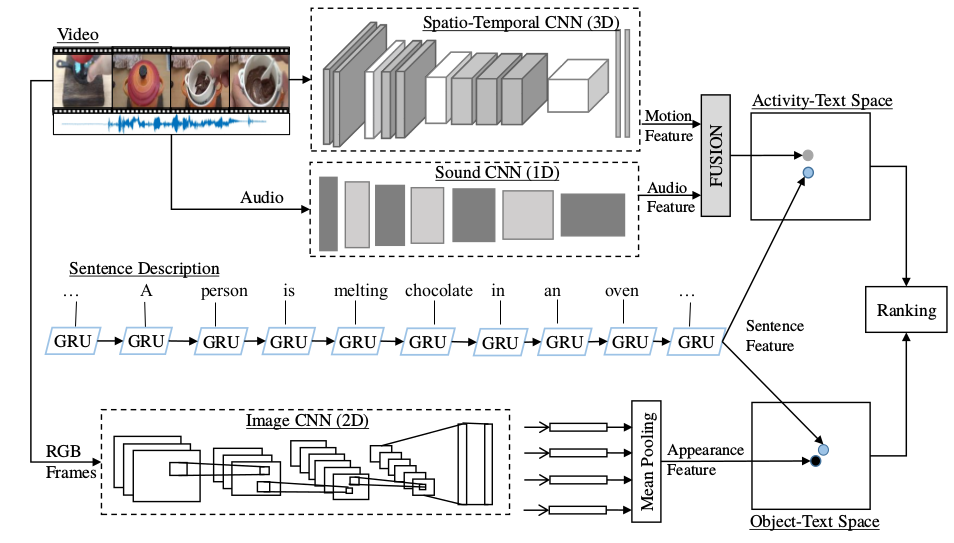
\includegraphics[width=\linewidth]{figures/related_mithun2018}
    \caption[Mithun等人~\cite{mithun2018learning}的活动-文本空间和物体-文本空间模型结构图]{\textbf{活动-文本空间和物体-文本空间模型结构图},来自~\cite{mithun2018learning}。}
    \label{fig:related_mithun2018}
\end{figure*}

而在视频片段检索领域,Yu等人~\cite{vsrel2020}使用了类似的做法,他们首先使用预训练的卷积神经网络VGG提取视频的帧图像特征,并使用平均池化的操作得到视频的物体特征,另外,他们还使用一个双流的卷积神经网络temporal segment network(TSN)~\cite{wang2016temporal}来提取视频的活动特征,该双流网络同时以帧图像和视频的光流作为输入。同样,他们单独地为这两类特征学习一个公共空间,并使用平均的方式后融合这两个公共空间。

考虑到视频具有非常复杂的信息,Miech等人在文献~\cite{miech2018learning}中提出的嵌入专家混合模型(Mixture of embedding experts,MEE) 使用多种视频的特征,包括ResNet-152对视频帧图像提取的物体特征,由I3D提取的视频的动作特征,由audio CNN提取视频的音频特征,他们还使用dlib框架~\footnote{http://dlib.net/}检测视频内的人脸并使用该框架里在人脸识别任务预训练的ResNet提取这些人脸特征,然后他们使用最大值池化对物体特征、动作特征和人脸特征在时间维度上进行池化,并使用NetVLAD对音频特征进行聚合,从而得到这视频级的这四种特征。而对于文本表示,他们先使用word2vec对句子的每个单词提取得到稠密特征,然后使用NetVLAD对单词特征进行聚合操作从而得到句子的特征表示。然后他们使用门控嵌入模块(Gated Embedding Module)来对这两种模态的特征进行处理,具体如公式~\ref{eq:gated-embedding-module}所示,
\begin{equation}
    \label{eq:gated-embedding-module}
    \begin{aligned}
        & Y_1 = W_1 X + b_1 \\
        & Y_2 = Y_1 \circ \sigma(W_2Y_1 + b_2) \\
        & Y = \frac{Y_2}{||Y_2||_2}
    \end{aligned}
\end{equation}
其中,$X$是输入的特征向量,$W_1$,$W_2$, $b_1$, $b_2$是可学习的参数,$\sigma$是sigmoid激活函数,$\circ$表示两个向量逐元素相乘。即对于每种视频特征,他们使用文本特征和该视频特征经过Gated Embedding Module处理,然后计算两种处理后的特征之间的余弦相似度,从而对于每对视频-文本对会产生四个余弦相似度,然后他们使用文本特征计算这四个相似度的权重,并根据该权重对这四个相似度加和得到视频-文本对的总相似度。他们的整体模型图如图~\ref{fig:related_miech2018}所示。

\begin{figure*}[tbh!]
    \centering
    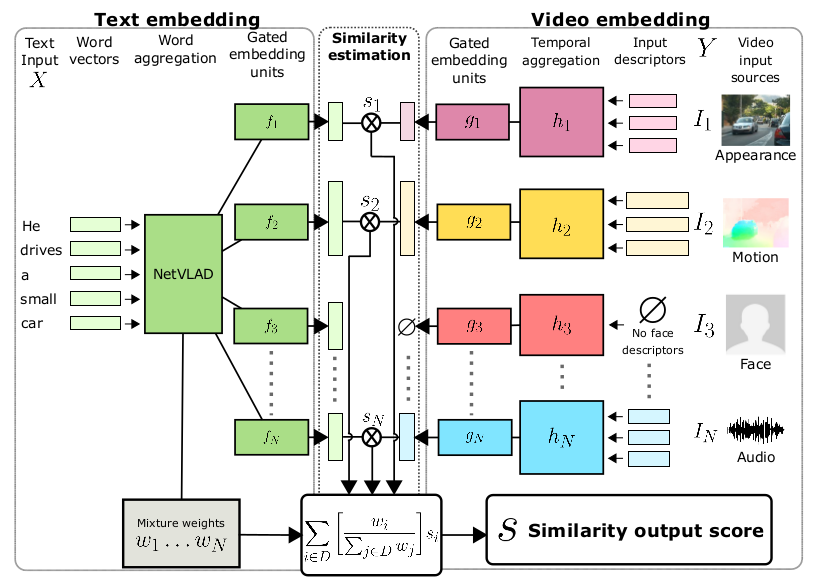
\includegraphics[width=\linewidth]{figures/related_miech2018}
    \caption[Miech等人~\cite{miech2018learning}的Mixture of embedding experts模型结构图]{\textbf{Mixture of embedding experts模型结构图},来自~\cite{miech2018learning}。}
    \label{fig:related_miech2018}
\end{figure*}

Liu等人~\cite{liu2019use}尽可能地挖掘了视频信息,他们提取了视频的物体特征、场景特征、动作特征、人脸特征、字符特征(optical character recognition,OCR)、言语(speech)特征和音频(audio)特征。他们首先使用深度卷积神经网络SENet-154~\cite{hu2019squeeze}模型提取视频帧图像的物体特征,在Places365~\cite{zhou2018places}数据上预训练的DenseNet-161~\cite{huang2017densely}提取帧图像的场景特征,双流卷积神经网络I3D提取连续帧图像的动作特征。而对于人脸特征,他们先使用人脸目标检测网络SSD~\cite{liu2016ssd}来提取帧图像中的人脸,然后再使用在VGGFace2~\cite{cao2018vggface2}数据上预训练的ResNet-50提取每个检测出的人脸的特征。对于OCR特征,他们先使用文本检测模型PixelLink~\cite{deng2018pixellink}来定位图像中的文本位置,然后每个文本框内的图像区域经过一个在文本识别数据Synth90K~\cite{liu2018synthetically}的模型~\cite{jakub-mm19}得到一序列字符串的文本,最后文本的每个单词的向量由预训练的word2vec模型提取。对于言语特征,他们使用谷歌云的API来对声音提取单词,然后得到的句子的单词的向量同样由word2vec模型提取。对于音频特征,他们使用在Youtube-8m~\cite{abuelhaija2016youtube}上预训练的audio CNN~\cite{hershey2017cnn}提取。最后,他们使用平均池化的方法来处理这些帧图像的物体特征、场景特征、动作特征和人脸特征,而使用NetVLAD的方法聚合OCR特征、言语特征和音频特征,从而最终得到视频级的相应的特征表示。为了融合所有的这些视频级特征,他们首先将这些特征做了线性投影,将所有特征转换到相同维度的特征,然后计算两两特征之间的关系,然后根据这个关系对转换后的特征进行缩放处理得到新的特征表示,使得有效的信息的权重加大,而冗余或者无效的信息被抑制,从而为模型提供了更加准确有效的特征作为输入。最终所有的视频特征都经过Gated Embedding Module~\cite{miech2018learning}处理,具体如公式~\ref{eq:gated-embedding-module},然后对所有的输出进行拼接并做L2规范化,得到最终的视频特征。而对于文本的表示,他们先用预训练的word2vec模型对句子的每个单词进行编码,然后这些单词编码再经过OpenAI-GPT~\cite{radford2018improving}模型,最后所有的输出通过NetVLAD进行聚合从而得到整个句子的编码,为了计算句子与视频的相似度,他们使用Gated Embedding Module为每个视频特征对句子编码进行处理,从而得到与视频特征维度相同的句子特征。他们使用余弦相似度计算句子与视频的相似度,并使用双向的排序损失函数(bidirectional marginal ranking loss)监督模型的训练。这种方法尽可能地使用了视频的信息,并且通过拼接的方法为每个视频特征学习跨模态计算的子空间,并将各个子空间的相似度相加融合。

Dong等人在文献~\cite{dong2018predicting}和Li等人在文献~\cite{li2019w2vv++}中通过拼接的方式融合了三种文本编码特征,即bag-of-words(bow)、word2vec和GRU,并且使用ResNet-152、ResNeXt-101为视频提取视觉特征。Dong等人~\cite{dong2018predicting}将拼接后的文本特征投影到视觉特征空间,在视觉特征空间中计算两种模态的距离。而Li等人~\cite{li2019w2vv++}将文本特征投影到视觉特征空间或将两种模态的特征同时投影到公共的隐空间,并在公共空间中计算文本和视频的余弦相似度。而Dong等人在文献~\cite{dong2019dual}进一步提出使用对偶的多层编码方式分别对文本和视频进行编码表示,他们的模型结构如图~\ref{fig:related_dong2019}所示,他们分别使用多层相似的编码方式对视频的帧特征和文本编码,即使用bow,bidirectional GRU(biGRU),并使用1D-CNN作用在bi-GRU的输出的所有隐藏层特征(biGRU-CNN),而在视频编码上,他们先使用ResNet-152对视频的帧图像提取视频特征,然后使用平均池化、biGRU和biGRU-CNN这三种方式对帧图像特征进行聚合得到三种层次的视频级特征,他们分别对文本的三种编码特征对视频的三种编码得到的视频特征进行拼接来表示文本和视频,最后使用全连接层对这两种模态的特征投影到公共的隐空间,从而在这个学习的隐空间中可以计算文本和视频的余弦相似度。

\begin{figure*}[tbh!]
    \centering
    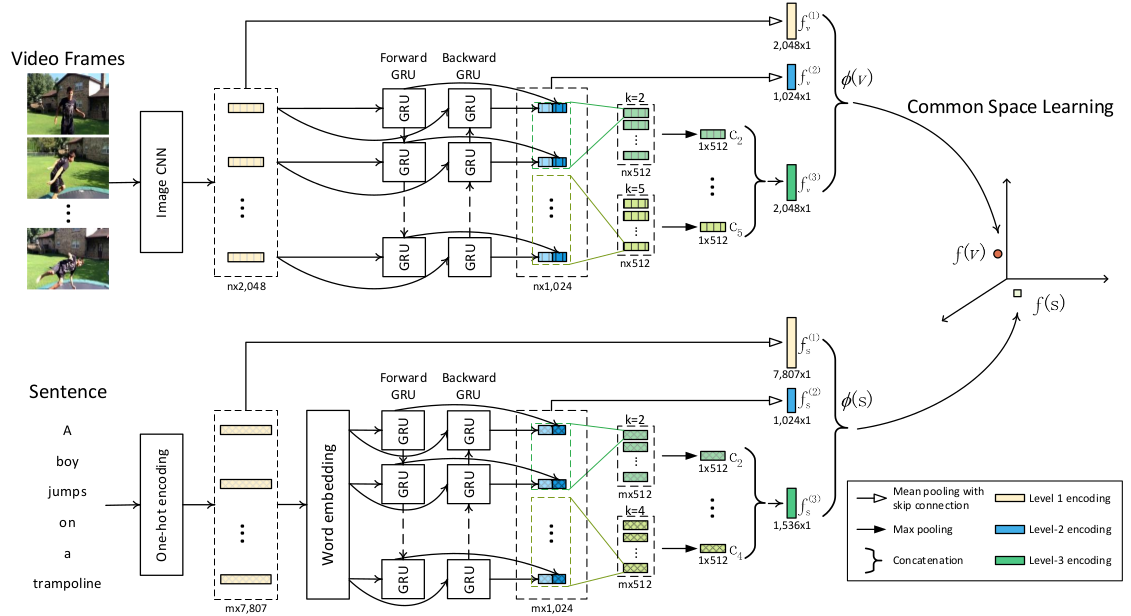
\includegraphics[width=\linewidth]{figures/related_dong2019}
    \caption[Dong等人~\cite{dong2019dual}的对偶编码网络模型结构图]{\textbf{对偶编码网络模型结构图},来自~\cite{dong2019dual}。}
    \label{fig:related_dong2019}
\end{figure*}

\section{本章小结}
本章首先回顾了近四年的TRECVID评测中的即席检索视频系统,可以发现即席视频检索技术是逐渐由基于概念的模型向基于完全深度学习的模型发展,近年来越来越多的即席视频检索技术是基于完全深度学习的方法,并取得了优秀的成绩。本文另一方面也回顾了一些基于文本的跨模态视频检索技术,因为文本与视频都是具有非常复杂语义信息的媒体数据,这些技术都采用了多种视频特征或者文本特征,并在同一个模型下融合这些特征,得到了更加出色检索的效果。

\chapter{算法设计}

\section{问题描述}
对于给定一个以自然句子表示的即席查询$s$,共包含$l$个单词$\{w_1,w_2,\cdots,\\w_l\}$,本文研究的目标是建立一个
视频检索系统,即从$n$个未被标注的视频集$\{v_1,v_2,\cdots,v_n\}$中搜索出与该查询相关的视频。问题的关键是构建
一个跨模态的相似度函数$f(s,v) \in \mathbf{R}$,使得相关的句子视频对$(s,v^+)$的相似度比不相关的句子视频对$(s,v^-)$
更大。相应地,在查询结果中相关的视频$v^+$会排在不相关的视频$v^-$的视频前。设$\mathbf{s}$和$\mathbf{v}$是查询与视频
在公共空间的向量化表示,则跨模态的相似度由余弦相似度得到:
\begin{equation}
    \label{eq:cosine-sim}
    \begin{aligned}
        f(s,v) := \frac{\mathbf{s}^T\mathbf{v}}{\left\| \mathbf{s} \right\| \cdot \left\| \mathbf{v} \right\|}
    \end{aligned}
\end{equation}

本研究着眼于查询表示学习,即由查询$s$获得在公共空间的向量$\mathbf{s}$,而视频可以像之前的工作一样由深度卷积网络得到
的特征或者概念向量表示。

\section{查询表示学习}
本研究是建立在W2VV~\cite{dong2018predicting}模型的基础上,W2VV模型原本是用在图像描述或者视频描述的检索任务上,共包含两个子网络,即一个
句子编码网络,把一个句子向量化和一个转换网络,将句子向量转换到视觉特征空间中。本研究对W2VV做如下改进:
\begin{itemize}
    \item 使用一个更好的句子编码策略。

    \item 使用一个更好的特征融合策略。

    \item 使用一个更好的目标函数用于模型训练。
\end{itemize}

\subsection{句子编码网络}
对于给定的一个句子$s$, 本研究同时使用三种编码技术对$s$进行向量化表示,即bag-of-words(bow),word2vec(w2v)词嵌入和
基于RNN的序列建模技术。对于bow编码技术,句子$s$的向量可以由如下式子得到:
\begin{equation}
    \label{eq:bow}
    \begin{aligned}
        \bm{\mathbf{bow}}(s) := (c(w_1,s),c(w_2,s),\cdots,c(w_m,s))
    \end{aligned}
\end{equation}
$c(w,s)$计算特定单词$w$在句子$s$中出现的次数,$m$表示给定词典的单词数量,本研究使用的词典由在训练数据中出现不少于5次
的单词组成,并且根据NLTK去掉其中的停用词。

对于一个给定的预训练w2v模型,用$\bm{\mathbf{e}}(w)$表示特定单词$w$的语义词嵌入向量,则w2v编码技术使用平均池化操作得到句子的向量:
\begin{equation}
    \label{eq:w2v}
    \begin{aligned}
        \bm{\mathbf{w2v}}(s) := \frac{1}{l}\sum^l_{i=1}e(w_i)
    \end{aligned}
\end{equation}
本研究使用一个500维的使用3000万张Flickr图像的英文标签训练的w2v模型~\cite{dong2018predicting},共支持超过170万个常见的单词向量化。

和W2VV相似,本研究同样使用Gated recurrent units(GRUs)~\cite{cho2014learning}作为序列模型对句子进行编码。GRU在特定的$t$时刻的输入
是句子中第$t$个单词的词嵌入向量,设为$\bm{\mathbf{e}}(w_t)$。该向量是从一个词嵌入矩阵$W_e$中对应的单词的词嵌入向量得到的。而GRU的输出,设为$h_t$
是通过联合当前词向量$\bm{\mathbf{e}}(w_t)$和GRU之前时刻的输出向量$h_{t-1}$由如下式子得到:
\begin{equation}
    \label{eq:gru}
    \begin{aligned}
        & z_t = \sigma_g(W_z e(w_t) + U_z h_{t-1} + b_z), \\
        & r_t = \sigma_g(W_r e(w_t) + U_r h_{t-1} + b_r), \\
        & \widetilde{h_t} = \sigma_h(W_h e(w_t) + U_h (r_t \circ h_{t-1}) + b_h), \\
        & h_t = (1-z_t) \circ h_{t-1} + z_t \circ \widetilde{h_t},
    \end{aligned}
\end{equation}
其中$z_t$ 和$r_t$表示在$t$时刻的更新门向量和重置门向量,$W$,$U$和$b$表示门的仿射转换参数,每个门输出前带有一个特定的激活函数,其中
$\sigma_g$表示sigmoid函数,$\sigma_h$表示双曲正切函数,操作$\circ$为两个向量的哈达玛积。

对于基于GRU的句子编码,W2VV只取最后时刻的输出向量,即$h_l$,而本研究通过对所有时刻的平均池化操作考虑所有的中间时刻的输出状态,即:
\begin{equation}
    \label{eq:gru-mean}
    \begin{aligned}
        \bm{\mathbf{gru}}(s) := \frac{1}{l}\sum^l_{i=1}h_i
    \end{aligned}
\end{equation}
对于GRU词典,与bow词典类似,但是GRU词典还包含停用词,因为它们在自然语句中含有有意义的上下文信息。

对于多种编码方式(bow, w2v, GRU)对句子进行编码,本文使用两种策略对这些编码方式进行融合,即:
\begin{itemize}
    \item W2VV++:使用与W2VV相同的方式,即向量拼接融合,即$\bm{\mathbf{ms}}(s)=[\bm{\mathbf{bow}}(s);\bm{\mathbf{w2v}}(s);\bm{\mathbf{gru}}(s)]$。本文将这种方式的模型称为W2VV++。

    \item TEE:三种编码方式互相独立,分别与视频向量。本文将这种方式的模型称为text encoding ensemble(TEE)。
\end{itemize}

\subsection{转换网络}
转换网络用于将之前的网络输出进行非线性仿射变换,即对于W2VV++模型,将$\bm{\mathbf{ms}}(s)$进行转换,对于TEE模型,分别对$\bm{\mathbf{bow}}(s)$,$\bm{\mathbf{w2v}}(s)$和$\bm{\mathbf{gru}}(s)$进行转换,
把文本编码得到的向量转换到一个公共空间,得到向量$\bm{\mathbf{s}}$,使得句子与视频的相关性可以由公式\ref{eq:cosine-sim}进行计算。
本文使用$k$层全连接层实现该转换网络。以W2VV++模型得到的文本编码向量$\bm{\mathbf{ms}}(s)$为例,对转换网络进行描述。第一层全连接层
的输出向量$\bm{\mathbf{fc_1}}(s)$由作用在向量$\bm{\mathbf{ms}}(s)$的仿射变换得到,即:
\begin{equation}
    \label{eq:fc-1}
    \begin{aligned}
        \bm{\mathbf{fc_1}}(s) = \sigma(A_1\bm{\mathbf{ms}}(s) + b_1)
    \end{aligned}
\end{equation}
其中$A_1$和$b_1$分别是全连接层的权重和偏移,$\sigma$是增强网络非线性的激活函数,本研究默认的激活函数是双曲正切函数。转换网络的剩余的全连接层计算如下公式:
\begin{equation}
    \label{eq:fc-k}
    \begin{aligned}
        \bm{\mathbf{fc_i}}(s) = \sigma(A_i\bm{\mathbf{fc_{i-1}}}(s) + b_i), i=2,...,k.
    \end{aligned}
\end{equation}
本研究的句子编码网络和转换网络是端到端地进行训练的,把网络的所有可学习的参数$\{W_z,U_z,b_z,W_r,U_r,b_r,W_h,U_h,b_h,W_e,A_1,b_1,\cdots,A_k,b_k\}$表示成$\theta$,相应地,相似度函数参数表示为$f(s,v;\theta)$。


\section{视频特征表示}
正如前文所言,本研究的目标在于查询表示学习,因此,对于视频的表示,本文简单地使用最先进的深度卷积网络通过过采样的方式提取视觉特征,
并且使用平均池化的操作获得视频的特征表示,如图\ref{fig:video-cnn-feat}所示。本文使用两个深度卷积网络模型进行视频的特征提取:
ResNext-101~\cite{}和ResNet-152~\cite{}。对于每个模型,本文选择模型的分类层输出作为特征,维度为2048维。
对于给定一个视频,本研究以0.5秒为间隔对视频的帧进行均匀采样。每张采样的图像的大小调整为$256\times256$,然后以$224\times224$大小
的窗口对该图像与其水平翻转得到的图像的四个角和中央进行裁剪,得到该图像的10张子图,这10张子图分别经过卷积网络提取特征并且进行
平均池化操作,得到该图像的特征表示。相应地,2048维的视频特征由图像特征进行平均池化得到。为了方便表示,本文将使用$ResNeXt$和$Resnet$
表示经过这两种卷积网络得到的视频特征,$ResNeXt$-$Resnet$表示这两种特征进行拼接得到的4096维的视频特征。

原则上,本研究的模型可以使用任何的视频特征表示,包括概念特征向量~\cite{}和3D卷积网络特征~\cite{}。

\begin{figure*}[tbhp!]
    \centering
    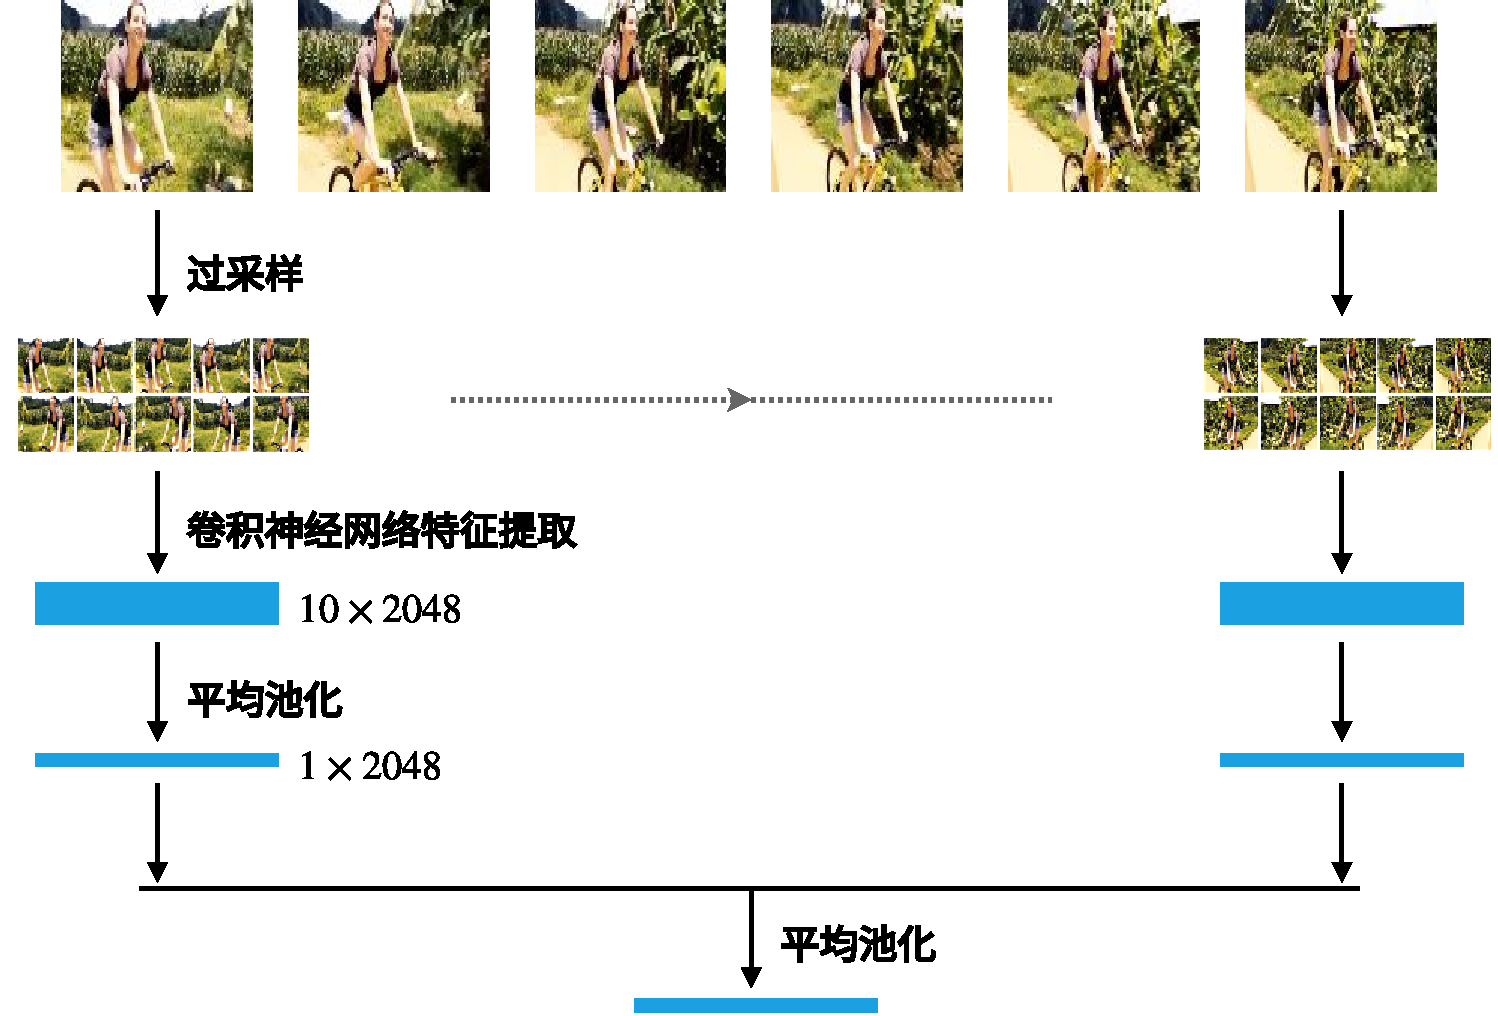
\includegraphics[width=\linewidth]{figures/video-cnn-feat}
    \caption[视频特征提取示例]{视频特征提取示例}
    \label{fig:video-cnn-feat}
\end{figure*}


\section{目标函数}




\section{公共空间表示}



,,

\chapter{实验}
\section{算法实现}
本文先使用OpenCV~\footnote{\url{https://opencv.org}}来对视频进行按照每0.5秒提取一张帧图像并保存到存储设备里,而提取帧图像的深度卷积特征是基于MxNet框架~\footnote{\url{http://mxnet.incubator.apache.org}},具体提取特征的代码项目video-cnn-feat~\footnote{\url{https://github.com/xuchaoxi/video-cnn-feat}}已经在github上开源。本文使用的两个预训练卷积神经网络(ResNet-152和ResNeXt-101)对实验数据提取的视觉特征~\footnote{\url{https://github.com/li-xirong/avs}}也已经在github上发布,每个视频的两种视觉特征都是2048维,而两种特征的拼接后的特征是4096维,每个视频的特征是由帧图像的特征进行平均池化操作得到的。

本文的W2VV++算法模型和SEA算法模型均使用PyTorch~\cite{pytorch}的深度学习框架实现,使用基于随机梯度下降法的RMSProp优化器对模型进行训练,优化器的学习率
根据实验经验设为0.0001,而其他参数使用默认值。为了防止训练时出现梯度爆炸,本研究把训练时的梯度降低L2范数倍。学习率在每次训练结束
后降为原来的0.99倍,如果模型在验证集上的性能连续三次没有提高则学习率降为原来的0.5倍。如果在验证集的性能连续10次没有提高,则模型训练
提前停止。本文最后测试的模型是在验证集上性能最好的模型。

模型训练的每个批次的大小为128对相关的句子-视频对,在每个批次给定的一个句子,本文把该批次里的其余剩余视频当作该句子的不相关视频,
即该句子与这些不相关视频构成负样本,而本文使用的最难负例来计算损失的策略,即选择这些负例中的最不相关的句子视频对来最后计算损失,
具体是余弦相似度最大的句子视频对作为最难负例。本文的W2VV++模型和SEA模型所有的公共跨模态空间的维度设为2048维。根据Faghri等人的文献~\cite{faghri2017vse++},目标函数公式\ref{eq:itrl}的超参数$\alpha$设为0.2。为了避免出现过拟合,本文在转换网络的全连接层使用概率为0.2的随机失活策略。本文的所有实验都在具有Nvidia GEFORCE GTX 1080Ti GPU显卡的服务器上进行。

\section{实验设置}
为了验证本文提出的W2VV++模型和SEA模型的有效性,本文在两个公开的视频数据基准线:MSR-VTT~\cite{msrvtt}和TRECVID AVS~\cite{awad2016trecvid}上进行实验。尽管MSR-VTT最初是用来研究视频描述生成的数据集,但是也有很多的基于文本的视频检索的工作~\cite{mithun2018learning,miech2019howto100m,dong2019dual,liu2019use,yu2018a}在该数据集上进行了尝试,TRECVID AVS是自从2016年以来在即席视频检索领域一个大型的非常重要的基准线~\cite{awad2016trecvid,awad2017trecvid,awad2018trecvid,awad2019trecvid},这两个基准线都有各自的特点。如表格~\ref{tab:datasets}所示,MSR-VTT的测试数据集的视频数量相对较少,只有2,990个视频,而每个视频具有20个句子描述,一共59,800个句子描述。而TRECVID AVS具有大量的测试视频,在2016、2017和2018年的测试里面有超过了33.5万个测试视频,在2019年有超过100万个测试视频。因此,在这两个数据基准线上进行详尽的实验可以公平地验证算法模型的有效性。

\begin{table} [tb!]
\renewcommand{\arraystretch}{1.2}
    \caption[本文实验所用的数据集]{\textbf{本文实验所用的数据集}。 本文所有的实验均用对应的训练集(train set)对模型进行训练,用对应的验证集(val. set)对模型进行验证,用对应的测试集(test set)对模型进行测试。}

\label{tab:datasets}
\centering
 \scalebox{0.87}{
 \begin{tabular}{@{} |l | l |r |r|r|r|r|@{}}
\hline


     \textbf{数据划分} & \textbf{数据名称} & \textbf{视频数} & \textbf{帧数} & \textbf{查询数} & \textbf{bow词典} & \textbf{GRU词典} \\
\hline
\multicolumn{7}{|l|}{\textbf{MSR-VTT 实验:}} \\
\hline
     \textit{train set} & \multirow{4}{*}{MSR-VTT~\cite{msrvtt}} & 6,513 & 197,648 & -- & 7,676 & 7,807 \\
\cline{1-1}  \cline{3-7} 
     \textit{val. set} &  & 497 & 15,347 & 9,940 & -- & -- \\
\cline{1-1}  \cline{3-7}
     \textit{test-full} &  & 2,990 & 92,467 & 59,800 & -- & -- \\
\cline{1-1}  \cline{3-7}
     \textit{test-1k}~\cite{yu2018a} &  & 1,000 & 30,932 & 1,000 & -- & -- \\

\hline
\hline
\multicolumn{7}{|l|}{\textbf{TRECVID 实验:}} \\
\hline
     \multirow{2}{*}{\textit{train set}} & MSR-VTT~\cite{msrvtt}  & 10,000 & 305,462 & --  & \multirow{2}{*}{11,147} & \multirow{2}{*}{11,282} \\
\cline{2-5}
     & TGIF~\cite{li2016tgif}   & 100,855 & 1,045,268 & -- &  & \\
\hline
     \textit{val. set} & TV16-VTT-dev~\cite{awad2016trecvid}  & 200 & 5,941 & 200  & -- & -- \\
\hline
     \specialcell{\textit{test set} for \\ TV16/17/18} & IACC.3~\cite{awad2016trecvid}  & 335,944 & 3,845,221 & 90 & -- & -- \\
\hline
     \specialcell{\textit{test set} for \\TV19} & V3C1~\cite{berns2019v3c1} & 1,082,649 & 7,839,450 & 30 & -- & -- \\
\hline
\end{tabular}
 }% end of scalebox
\end{table}


%\begin{table} [tbh!]
%    \caption[AVS数据集]{这是AVS数据集的基本统计描述}
%    \label{tab:avs-dataset}
%    \centering
%    \scalebox{0.96}{
%        \begin{tabular}{@{}l r r r r r@{}}
%            \toprule
%            \textbf{数据集名称} & \textbf{镜头数} & \textbf{帧数} & \textbf{句子数} & \textbf{bow词典大小} & \textbf{GRU词典大小} \\
%            \hline
%            \emph{训练集:} & & & & & \\
%            MSR-VTT & 10,000 & 305,462 & 200,000 & \multirow{2}{*}{11,147} & \multirow{2}{*}{11,282} \\
%            TGIF & 100,855 & 1,045,268 & 124,534 & & \\
%            \hline
%            \emph{验证集:} & & & & & \\ 
%            TV16-VTT-train & 200 & 5,941 & 200 & - & - \\
%            \hline
%            \emph{测试集:} & & & & & \\
%            IACC.3 & 335,944 & 3,845,221 & - & - & - \\
%            V3C1 & 1,082,649 & 7,839,450 & - & - & - \\
%            \bottomrule
%        \end{tabular}
%    }
%\end{table}



\subsection{MSR-VTT 实验设置} \label{ssec:setup-msrvtt}
\textbf{数据划分}:本文根据MSR-VTT数据官方的数据划分,共分为三个没有交集的子集作为训练集、验证集和测试集,其中训练数据包含6,513个视频,130,260个句子描述,而验证集包含497个视频,9,940个句子描述作为查询,测试集包含2,990个视频,59,800个句子描述作为查询。而在文献~\cite{liu2019use,miech2019howto100m,yu2018a}中,这些工作在原来的测试集里随机采样了1,000个视频作为一个更小的测试集,而查询句子也进行了随机采样得到1,000个句子,每个视频对应一个句子描述。本文为了与这些工作进行公平的比较,也使用了这个更小的测试集,命名为\textit{test-1k},而原来的完整测试集命名为\textit{test-full}。

\textbf{性能指标}:根据之前的工作~\cite{dong2019dual,mithun2018learning},本文在MSR-VTT实验报告的指标为R@k, k=1,5,10,表示测试查询样例在前k个查询结果中至少有一个相关视频的百分比,该值越大模型效果越好,排序中位数(Median rank, Med r),表示在查询结果中第一个相关视频的排序的中位数,该值越小模型效果越好,和平均精度均值(Mean Average Precision, mAP)作为模型整体性能的指标,在验证集上也是使用mAP作为选择最优模型的指标。

\subsection{TRECVID 实验设置} \label{ssec:setup-tv}

\textbf{训练集}:如表格~\ref{tab:datasets}所示,本文的TRECVID实验使用MSR-VTT~\cite{msrvtt}和TGIF~\cite{li2016tgif}两个数据结合作为训练集。MSR-VTT数据包含1万个网络视频片段和20万个描述视频片段内容的句子,即每个视频片段有20个描述句子。
本文每段MSR-VTT的视频每半秒提取一帧的频率进行均匀采样,共生成305,462张帧图像。而TGIF数据包含超过10万张动图和12万个描述动图内容的句子,本文同样对每个动图进行均匀采样,共生成1,045,268张帧图像。

\textbf{验证集}:本文使用TRECVID 2016 Video-to-Text任务~\cite{awad2016trecvid}的训练集作为验证集,命名为TV16-VTT-dev,用于模型训练阶段的对最优模型的选择。这个集合共包含200个视频,每个视频含有2个描述视频内容的句子。对于每个视频,本文选择第一个句子作为该视频的文本查询,
而剩余的199个视频则是该查询的不相关视频。相应地,本文使用平均精度均值(mAP)作为评价模型在该验证集以文本检索视频的性能指标。

\textbf{视频测试集}:本文使用TRECVID的AVS任务在2016年至2018年使用的官方测试视频集IACC.3~\cite{awad2016trecvid}和在2019年使用的官方测试视频集V3C1~\cite{berns2019v3c1}。IACC.3数据集包含4,953个网络视频(600小时),视频的时长从6.5分钟到9.5分钟,平均时长为7.8分钟。
官方已经对视频做了自动镜头边界检测,共生成335,944个视频片段,用户的检索目标是这些独立的视频片段。本文同样对每个视频片段进行均匀采样,共生成3,845,221张帧图像。而TRECVID AVS 2019年使用的V3C1视频集是一个更大的未被标注的视频数据集,共包含了7,475个网络视频(1000小时),平均每个视频长为8分钟,同样,TRECVID官方对视频做了镜头自动分割,共被划分为1,082,649个视频片段。本文使用均匀采样对这些视频片段提取帧图像,共生成7,839,450张帧图像。

\textbf{查询测试集}:TRECVID的AVS任务每年定义30个查询来进行测试,每个查询是自然语言的句子形式,具有不同的长度和不同的语义难度。
例如“Find shots of palm trees”,“Find shots of a man with beard and wearing white robe speaking and gesturing to camera”和
“Find shots of a truck standing still while a person is walking beside or in front of it”。所有的查询均以“Find shots of”的短语开头,因此在测试时可以很容易地去掉而关注查询的主体部分。

\textbf{性能指标}:本文使用TRECVID AVS任务的官方评测指标,推测平均准确率(inferred average precision, infAP)~\cite{awad2016trecvid,awad2017trecvid,awad2018trecvid,awad2019trecvid}作为模型的评价指标,而模型的总体性能是所有测试查询样例的infAP分数的平均值,该值越高,模型的视频检索效果越好,本文以2016-2019年的infAP的平均值(AVG)作为模型在TRECVID上的整体性能。


\section{实验结果}
本文从消融实验和与先进方法的比较实验两个方面验证本文提出的W2VV++模型和SEA模型的有效性,消融实验可以验证不同模块对于模型的作用,从而验证本文提出的对于特定模块的改进的有效性,与目前的先进方法进行比较实验可以验证本文所提出的算法模型在即席视频检索领域具有优越性。

\subsection{消融实验}
\textbf{视频特征的选择}:本文比较了三种特征的选择,即$ResNeXt$,$ResNet$和$ResNeXt$-$ResNet$,分别表示ResNeXt-101特征,ResNet-152特征和这两个特征的拼接组成的特征。如表格~\ref{tab:tee_vs_w2vvpp}所示,对于模型W2VV++和SEA,使用ResNeXt-101的视频的特征比使用ResNet-152的效果好,而使用这两个特征拼接组成的$ResNeXt$-$ResNet$视频特征可以进一步提高这两个模型的性能。对于相同的视频特征,本文提出的W2VV++模型和SEA模型都比基础模型W2VV的效果好,其中SEA模型的效果最好。本文接下来的实验均以拼接的特征$ResNeXt$-$ResNet$进行实验,除非特别说明。



\begin{table*}[tbh!]
\normalsize
\renewcommand\arraystretch{1.2}
\centering
\caption{\textbf{Joint evaluation of sentence encoders and their assembly models, \ie W2VV++ and the proposed \emph{SEA}, on MSR-VTT and TRECVID}. Numbers are shown in percentages, with top performers highlighted in \best{bold} font. For a given setup of sentence encoders, relative improvement of SEA over its W2VV++ counterpart is given in parentheses, showing that SEA is consistently better.}
\label{tab:tee_vs_w2vvpp}
\scalebox{0.75}{
\begin{tabular}{@{}|l | l | r | r | r | r | l|| r | r | r | r | l|@{}}
\hline
\multirow{2}{*}{\textbf{模型}} & \multirow{2}{*}{\textbf{视频特征}} & \multicolumn{5}{c||}{\textbf{MSR-VTT} (test-full)} & \multicolumn{5}{c|}{\textbf{TRECVID} (指标: infAP)}  \\
\cline{3-12}
 & & \textit{R@1} & \textit{R@5} & \textit{R@10} & \textit{Med r} & \textit{mAP} & \textit{TV16} & \textit{TV17} & \textit{TV18} & \textit{TV19} & \textit{AVG}  \\

\hline
\multirow{3}{*}{W2VV++} & $ResNet$ &  &  &  &  & & & & & & \\

\cline{2-12}
 & $ResNeXt$ &  & & & & & 14.0 & 17.1 & 10.3 & & \\

\cline{2-12}   
 & $ResNeXt$-$ResNet$ & 11.1 & 29.6 & 40.5 & 18 & 20.6  & 16.2 & 22.3 & 10.1 & 13.9 & 15.6 \\

\hline
\multirow{3}{*}{SEA} & $ResNet$ & & & & & & & & & & \\

\cline{2-12}
 & $ResNeXt$ & & & & & & & & & & \\

\cline{2-12}
    & $ResNeXt$-$ResNet$ & \best{12.2} & \best{31.9} & \best{43.1} & \best{15} & \best{22.1} & 15.0 & \best{23.4} & \best{12.2} & \best{16.6} & \best{16.8} \\

\hline 

\end{tabular}
}
\end{table*}


\textbf{目标函数}:本文提出的W2VV++模型在W2VV模型的基础上对目标函数和GRU编码器的使用做了改进,即使用ITRL目标函数替换原来的均方误差(MSE)目标函数,使用GRU输出的所有隐藏层状态的平均替换原来的只取GRU输出的最后时刻的隐藏层状态。如表格~\ref{tab:loss_fusion}前三行所示,W2VV$_{ITRL}$表示在模型W2VV的基础上只将ITRL替换MSE,由结果可以看出,使用ITRL目标函数可以大幅提高基于文本的视频检索模型的性能,而本文提出的W2VV++可以进一步提高视频检索的效果。对于SEA的目标函数选择,本文已经在图~\ref{fig:negative-examples}定性地分析了多目标函数(combined loss)融合文本编码器的比单目标函数(single loss)的方式更好,本文通过实验进一步验证了这个结论。如表格~\ref{tab:loss_fusion}的最后两行显示,在两个数据集上,多目标函数的方式都比单目标函数的方式的效果好。



\begin{table*}[tbh!]
\normalsize
\renewcommand\arraystretch{1.2}
\centering
    \caption[在MSR-VTT和TRECVID上联合评测目标函数不同的模型和文本编码器融合方式不同的模型]{\textbf{在MSR-VTT和TRECVID上联合评测目标函数不同的模型和文本编码器融合方式不同的模型}。评价指标除了中位排序数Med r均以百分数的形式显示(\%),其中最好的结果用\best{粗体}标出。本文提出的W2VV++模型对基础模型W2VV的目标函数的改进起到了很大的作用,并且也更有效地使用了GRU编码器,而使用多空间多目标函数融合文本编码器的SEA模型的性能最好。}
\label{tab:loss_fusion}
\scalebox{0.79}{
\begin{tabular}{@{}|l | r | r | r | r | l|| r | r | r | r | l|@{}}
\hline
\multirow{2}{*}{\textbf{模型}} & \multicolumn{5}{c||}{\textbf{MSR-VTT} (test-full)} & \multicolumn{5}{c|}{\textbf{TRECVID} (指标: infAP)}  \\
\cline{2-11}
 & \textit{R@1} & \textit{R@5} & \textit{R@10} & \textit{Med r} & \textit{mAP} & \textit{TV16} & \textit{TV17} & \textit{TV18} & \textit{TV19} & \textit{AVG}  \\

\hline
W2VV & 1.1 & 4.7 & 8.0 & 240 & \textcolor{white}{0}3.7 & 1.3 & 0.8 & 0.4 & 0.2 & \textcolor{white}{0}0.7 \\

\cline{1-11}
W2VV$_{ITRL}$ & 9.7 & 27.2 & 37.3 & 22 & 18.7 & 13.8 & 18.8 & 10.5 & 11.4 & 13.6 \\

\cline{1-11}
W2VV++ &  11.1 & 29.6 & 40.5 & 18 & 20.6  & \best{16.2} & 22.3 & 10.1 & 13.9 & 15.6 \\

\cline{1-11}
Transformed W2VV++ & 10.5 & 28.2 & 39.0 & 20 & 19.5 & 13.9 & 20.2 & 10.2 & 13.5 & 14.5 \\

\cline{1-11}
Model averaging & 12.0 & 31.8 & 42.9 & 16 & 22.0  & 14.9 & 21.9 & 11.6 & 15.4 & 16.0 \\

\cline{1-11}
SEA single loss & 11.8 & 31.0 & 42.0 & 17 & 21.5  & 14.7 & 21.8 & 11.2 & 14.7 & 15.6 \\

\cline{1-11}
SEA combined loss & \best{12.2} & \best{31.9} & \best{43.1} & \best{15} & \best{22.1}  & 15.0 & \best{23.4} & \best{12.2} & \best{16.6} & \best{16.8} \\


\hline 

\end{tabular}
}
\end{table*}




\textbf{文本编码器融合}:因为单个的文本编码器的输出维度差异很大,从500维($e_{w2v}$)到多达一万多维($e_{bow}$),像W2VV模型和本文提出的W2VV++模型直接简单地拼接这些文本编码器的方法不一定是最优的,而本文继续实现了两种融合方法,从而验证本文的提出的SEA模型可以更加有效地利用多个文本编码器:\\
$\bullet$ Transformed W2VV++:本文使用只有一层全连接层和激活层转换网络对W2VV++的每个编码器进行转换,使得每个编码器输出的句子向量的维度都是2048维,然后再融合这些转换后的编码器向量组成句子的向量化表示,然后再用转换网络把句子向量投影投公共空间。这种方式可以在编码器拼接时每个句子编码向量的维度一样。同样,这种方式也是通过端到端地对模型进行训练。  \\
$\bullet$ 模型平均后融合(Model averaging):先使用W2VV++模型对每个编码器单独训练好一个独立的模型,本文使用三个不同的文本编码器,因此会有三个独立的模型, 然后查询句子与视频的跨模态相似度由在这三个模型分别计算的跨模态相似度取平均得到。

如表格~\ref{tab:loss_fusion}所示,Transformed W2VV++模型相对于W2VV++的效果更差了,说明了对文本编码器输出的句子向量做维度的变化会导致编码器输出的信息丢失,而Model averaging的效果比W2VV++的效果更好,进一步说明了为多个编码器学习多个公共空间的比单个公共空间的更好,但Model averaging的效果不如本文提出的多空间多目标函数SEA模型,说明了在同一个模型里学习多空间是更优的方式。


\subsection{与先进方法的比较实验}
本文在MSR-VTT和TRECVID两个基准线都与当前的先进的视频检索算法进行了比较。

\textbf{在MSR-VTT上的先进方法} 。本文和下列的六个当前先进的算法模型进行了对比,分别是只在test-1k测试集上评测的算法~\cite{miech2019howto100m,yu2018a}和只在整个测试集test-full上评测的算法~\cite{mithun2018learning},以及在这两个测试集上评测的算法~\cite{dong2019dual,faghri2017vse++,liu2019use}。本文下面突出介绍这些算法所使用的文本编码器:\\
$\bullet$ JSFusion~\cite{yu2018a}: 使用双向的长短期记忆网络(bi-LSTM)作为文本编码器。 \\
$\bullet$ VSE++~\cite{faghri2017vse++}: 使用GRU作为文本编码器。 \\
$\bullet$ Mithun 等人~\cite{mithun2018learning}: 使用GRU作为文本编码器。 \\
$\bullet$ Miech 等人~\cite{miech2019howto100m}: 使用一维卷积神经网络(1D-CNN)作为文本编码器。 \\
$\bullet$ Dual Encoding~\cite{dong2019dual}: 在文本端和视频端同时使用多层对偶的编码策略。\\
$\bullet$ CE~\cite{liu2019use}: 使用 NetVLAD 作为文本编码器。\\
这些算法除了~\cite{miech2019howto100m},都在MSR-VTT的官方训练数据上进行模型的训练,而~\cite{miech2019howto100m}先在1亿的视频里进行预训练,然后在MSR-VTT数据上对模型进行微调。

本文在表格~\ref{tab:sota-msrvtt}展示了目前在MSR-VTT上完整的测试集test-full和test-1k上的先进算法的结果。为了方便对比,这些算法的结果直接从原始的论文中引用,除了VSE++~\footnote{\url{https://github.com/fartashf/vsepp}}和Dual Encoding~\footnote{\url{https://github.com/danieljf24/dual_encoding}}这两个算法,本文使用作者公开的代码并用本文所使用的视频特征$ResNeXt$-$ResNet$对模型进行了重新训练。在这些先进的算法中,CE模型在test-1k上的表现最好,而在完整测试集test-full上,Dual Encoding模型的效果最好。在test-1k上,本文提出了SEA算法模型在R@1上最好,而在R@5,R@10和Med r三个指标上与最好的CE模型相当。而在完整的测试集test-full上,本文提出的W2VV++模型和SEA模型均超过了这些先进方法,其中SEA模型在所有指标都是表现最好的。考虑到效果较好的CE模型使用了物体特征、场景特征、动作特征、人脸特征、字符特征、言语特征和音频特征来表示视频,而我们仅使用了物体特征,显然本文提出的算法模型更有优势。



\begin{table}[tb!]
\normalsize
\renewcommand\arraystretch{1.2}
\centering
    \caption[在MSR-VTT上目前先进的基于文本的视频检索算法]{\textbf{在MSR-VTT上目前先进的基于文本的视频检索算法}。 这些先进的算法都是从原论文引用,除了VSE++~\cite{faghri2017vse++}和Dual Encoding~\cite{dong2019dual}这两个算法是使用他们公开的源代码并用与本文实验相同的$ResNeXt$-$ResNet$视频特征重新训练,在test-1k测试集上,本文提出的SEA算法在R@1上最好,而在R@5,R@10 和 Med r 三个指标上与 CE~\cite{liu2019use}算法相当,而在完整的测试集test-full上本文提出的W2VV++和SEA算法都超过了这些先进算法,其中 SEA 模型在所有指标都是表现最好的。}
\label{tab:sota-msrvtt}
\scalebox{0.9}{
\begin{tabular}{@{}|l |l | r | r | r | r | r|@{}}
\hline
\textbf{测试集} & \textbf{模型} & \textbf{R@1} & \textbf{R@5} & \textbf{R@10} & \textbf{Med r} & \textbf{mAP} \\
\hline
\multirow{4}{*}{\textit{test-1k}~\cite{yu2018a}} & JSFusion~\cite{yu2018a} & 10.2 & 31.2 & 43.2 & 13 & n.a. \\
\cline{2-7}
%& Miech \etal~\cite{miech-iccv19} & 12.1 & 35.0 &  48.0 & 12 & n.a. \\
& VSE++~\cite{faghri2017vse++} & 15.2	& 37.7 & 50.1 & 10 & 26.0 \\
\cline{2-7}
& Miech \etal~\cite{miech2019howto100m} &14.9 & 40.2 &  52.8 & 9  & n.a. \\
\cline{2-7}
& UniViLM~\cite{luo2020univilm} & 15.4 & 39.5 & 52.3 & 9 & n.a. \\
\cline{2-7}
& Dual Encoding~\cite{dong2019dual} & 18.8 & 44.4 & 57.2 & 7 &31.6 \\
\cline{2-7}
& CE~\cite{liu2019use}  & 20.9 & \best{48.8} & \best{62.4} & \best{6} & n.a. \\
\cline{2-7}
& \multicolumn{6}{l|}{本文提出的模型:} \\
\cline{2-7}
& W2VV++ & 18.9 & 45.3 & 57.5 & 8 & 31.6 \\
\cline{2-7}
& \tea & \best{22.1} & 48.6 & 62.3 & \best{6}	& \best{34.9} \\ 

\hline
\hline
\multirow{5}{*}{\textit{test-full}} & Mithun \etal~\cite{mithun2018learning} & 7.0 & 20.9 & 29.7 & 38 & n.a. \\
\cline{2-7}
& VSE++ & 8.7 & 24.3 & 34.1  & 28 & 16.9 \\
\cline{2-7}
& CE & 10.0 & 29.0 & 41.2 &	16 & n.a. \\
\cline{2-7}
& Dual Encoding & 11.1 & 29.4 & 40.3 & 19 & 20.5 \\
\cline{2-7}
& \multicolumn{6}{l|}{本文提出的模型:} \\
\cline{2-7}
& W2VV++ & 11.1 & 29.6 & 40.5 &	18	& 20.6 \\
\cline{2-7}
& \tea & \best{12.2} & \best{31.9} & \best{43.1} & \best{15} & \best{22.1} \\
\hline
\end{tabular}
}
\end{table}


\textbf{在TRECVID AVS上的先进方法}。本文与在每年TRECVID AVS评测中前三的算法进行比较,并且本文还与VSE++和Dual Encoding这两个算法进行对比实验,这两个算法经过如第\ref{ssec:setup-tv}节的描述进行了重新训练,本文还与使用了bow作为文本编码器的VideoStory算法~\cite{habibian2017video2vec}进行了对比。

本文在表格~\ref{tab:sota-tv}展示了2016年至2019年在TRECVID上即席视频检索算法的性能。本文提出的SEA算法在TRECVID上的整体效果最好。考虑到之前在TRECVID评测上效果最好的模型都使用了对很多单模型进行平均后融合操作~\cite{snoek2017university,li2018renmin,wu2019hybrid},有的甚至用接近100个单模型~\cite{ueki2019waseda},而本文提出的SEA算法仅使用一个单模型就达到了目前最好的性能,这在即席视频检索领域是很大的一次改进。





\begin{table}[tb!]
\normalsize
\renewcommand\arraystretch{1.2}
\centering
\caption[在TRECVID即席视频检索任务上的先进算法比较]{\textbf{在TRECVID即席视频检索任务上的先进算法比较}。 本文提出的SEA算法超过了之前的检索算法,是目前在TRECVID即席视频检索任务上性能最好的算法。}
\label{tab:sota-tv}
\scalebox{0.9}{
\begin{tabular}{@{}|l | l | l | l | l | c| @{}}
\hline
\textbf{Model} & \textbf{TV16} & \textbf{TV17} & \textbf{TV18} & \textbf{TV19} & \textbf{AVG} \\
\hline 
\multicolumn{6}{|l|}{TRECVID 前三名:}  \\
\cline{2-6}
第一名 & \textcolor{white}{0}5.4~\cite{le2016nii} & 20.6~\cite{snoek2017university} & 12.1~\cite{li2018renmin} & 16.3~\cite{wu2019hybrid} & n.a. \\ 
第二名 & \textcolor{white}{0}5.1~\cite{foteini2016iti} & 15.9~\cite{ueki2017waseda} & \textcolor{white}{0}8.7~\cite{huang2018informedia} & 16.0~\cite{li2019renmin} & n.a.\\
第三名 & \textcolor{white}{0}4.0~\cite{liang2016inf} & 12.0~\cite{nguyen2017vireo} &  \textcolor{white}{0}8.2~\cite{bastan2018ntu} & 12.3~\cite{ueki2019waseda} & n.a.\\
\hline
VideoStory~\cite{habibian2017video2vec} & \textcolor{white}{0}8.7 & 15.0 & n.a. & n.a. & n.a. \\
\hline
VSE++~\cite{faghri2017vse++} & 13.5 & 16.3  & 10.6 & \textcolor{white}{0}9.8  & 12.6 \\ 
\hline
Dual Encoding~\cite{dong2019dual} & \best{16.5} & 22.8 & 11.7 & 15.2 & 16.6 \\
\hline
W2VV++ & 16.2 & 22.3 & 10.1 & 13.9 & 15.6   \\
\hline
\tea  & 15.0 & \best{23.4} & \best{12.2}  & \best{16.6} & \best{16.8} \\
\hline 
%Dual Encoding + \tea & \best{17.3} & \best{25.0} & \best{12.8} & \best{17.1} & \best{72.2} \\
%\hline
\end{tabular}
}
\end{table}



%\input{table-w2vvpp-avs}



\section{即席视频检索结果展示}


\section{本章小结}
在本章,我们详细地在两个公开的数据集MSR-VTT~\cite{msrvtt}和TRECVID AVS任务数据集~\cite{awad2016trecvid}上评测了在本文提出的W2VV++算法模型和SEA算法模型的有效性。本文提出的W2VV++算法在原来的W2VV算法~\cite{dong2018predicting}的基础上进行了改进,即使用了ITRL目标函数替换原来的MSE函数,使用GRU编码器输出的所有隐藏层状态的平均,而不仅是使用GRU编码器最后时刻的输出状态,通过消融实验证明了这两个改进在即席视频检索上都是有效的,而使用ITRL目标函数提高的效果最明显。本文提出的的SEA算法在W2VV++的基础上使用多空间多目标函数的方式融合多个文本编码器,通过消融实验验证了这种多空间多目标函数的方式可以非常有效地融合不同的文本编码器。通过与目前在视频检索上先进的算法进行对比,证明了W2VV++算法和SEA算法具有很大的优越性,其中单模型的SEA在TRECVID上进行评测的通过多个模型后融合的方法取得的结果,这在即席视频检索上是一个很大的进步。

%要插入本科签名的最后一个章节,插入命令使用\input{}
\chapter{总结与展望}

\section{总结}
    本文围绕即席视频检索这个十分重要且很有挑战的问题,本文通过调研了目前主流的视频检索算法,总结了这些算法都有的三个关键组件,即文本表示、视频表示和公共空间表示。本文基于深度学习技术,对原本用于图文检索的W2VV算法的文本表示和公共空间进行表示改进,提出了适用于即席视频检索任务上的W2VV++深度学习算法,并且不同于以往基于概念的方法,W2VV++是不依赖与概念建模的,并且可以对模型进行端到端的训练,因此可以联合优化文本表示和在公共空间中的跨模态相似度计算。在W2VV++算法的基础上,本文继续探究文本特征表示的融合策略,提出了多空间学习的SEA算法,本文通过科学系统的评测,验证了这两个算法在视频检索上具有很大的优越性。本文的研究成果可以概括如下:
    \begin{enumerate}[\hspace{2em}1.]
        \item 本文首先对即席视频检索领域的权威评测TRECVID上的前三名的算法围绕三个关键组件进行了综述:即从文本表示、视频表示和公共空间表示这三个在跨模态检索上的关键方面总结了这些算法的优势和不足。然后本文从这三个方面还列举并分析了目前主流的基于文本的视频检索算法。
        \item 本文分析了原本用于图文检索的W2VV算法的不足,并针对这些不足进行了改进,即使用更好的目标函数ITRL监督模型训练和使用GRU输出的所有隐藏层状态的平均作为文本表示的一部分,并适用在即席视频检索任务上,通过系统的实验证明了这两个改进对算法性能的提升都起到了关键作用。
        \item 本文继续研究的多空间学习的SEA算法相对W2VV++的效果更进一步,证明了通过多空间学习的方式融合不同的文本编码器的效果比直接拼接的方式更好,而且SEA算法在MSR-VTT和TRECVID两个数据上都取得了目前最好的视频检索的性能。

    \end{enumerate}


\section{展望}
    本文的研究内容仍然有很多可以继续研究并完善的地方,本文在这里列举,希望对读者有所启发:

    \begin{enumerate}[\hspace{2em}1.]
        \item 本文通过对视频的帧特征通过平均池化的操作来获得视频级的特征,这种简单的方法会导致视频时序信息的丢失和视频内关键内容的重要性减弱,对视频中的时空信息的深入挖掘和对视频关键内容的识别对视频的检索和理解具有重要的研究意义。

        \item 本文使用的文本编码器bag-of-words,word2vec和基于循环神经网络的GRU都不是现在最前沿的文本表示方法,探究更好的文本编码器,如目前在多项自然语言处理任务上取得突破成果的BERT模型,在跨模态的视频检索上的性能也具有重要的研究价值。

        \item 本文所使用的目标函数ITRL中只考虑了文本与视频的相似度关系,实际上文本与文本的相似性、视频之间的相似性对基于文本的视频检索效果都会有影响,因此如何将这些相似性联系起来一起作为优化目标是值得研究的问题。

    \end{enumerate}


%本科签名
%\autograph


%参考文献
%\bibliographystyle{ref/rucbib}
\bibliographystyle{unsrt}
\bibliography{ref/reference}
%\nocite{*}
\addcontentsline{toc}{chapter}{参考文献}

%附录
\appendix
\chapter{即席视频检索结果展示} \label{app:app-a}
\begin{figure*}[tbh!]
    \centering
    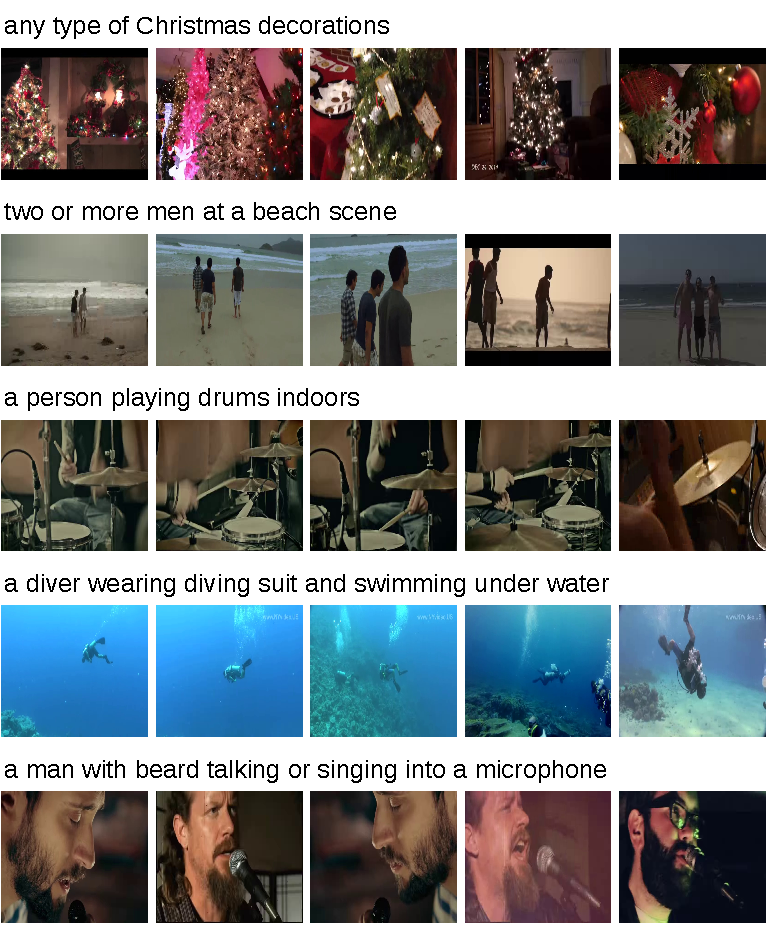
\includegraphics[width=\linewidth]{figures/search_result_1}
    \caption[SEA模型在V3C1上的即席视频检索结果展示]{\textbf{SEA模型在V3C1上的即席视频检索结果展示。这里的查询句子均来自TRECVID AVS评测,展示了检索结果的前5个视频。}}
    \label{fig:search_result_1}
\end{figure*}

\begin{figure*}[tbh!]
    \centering
    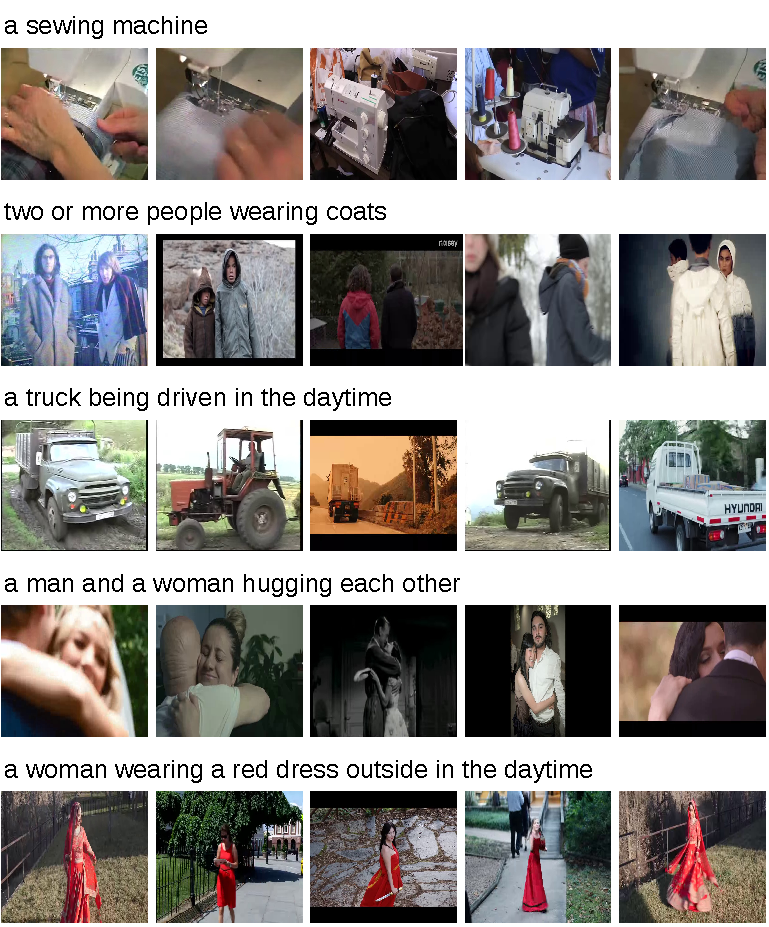
\includegraphics[width=\linewidth]{figures/search_result_2}
    \caption[SEA模型在V3C1上的即席视频检索结果展示(续)]{\textbf{SEA模型在V3C1上的即席视频检索结果展示(续)。这里的查询句子均来自TRECVID AVS评测,展示了检索结果的前5个视频。}}
    \label{fig:search_result_2}
\end{figure*}



%致谢
\begin{acknowledge}%致谢
感谢
\end{acknowledge}


\begin{achievement}%成果
    \begin{enumerate}[1.]
        \item 已发表的论文
            \begin{enumerate}[(1)]
                \item Xirong Li, \textbf{Chaoxi Xu}, Xiaoxu Wang, Weiyu Lan, Zhengxiong Jia, Gang Yang, Jieping Xu: COCO-CN for Cross-Lingual Image Tagging, Captioning and Retrieval. IEEE Transactions on Multimedia (T-MM), 2019. (SCI,CCF B类期刊,影响因子5.452)
                \item Jianfeng Dong, Xirong Li, \textbf{Chaoxi Xu}, Shouling Ji, Yuan He, Gang Yang, Xun Wang: Dual Encoding for Zero-Example Video Retrieval. IEEE Conference on Computer Vision and Pattern Recognition (CVPR), 2019. (CCF A类会议,计算机视觉顶级会议)
                \item \textbf{Chaoxi Xu}, Xiangjia Zhu, Wenwen He, Yi Lu, Xixi He, Zongjiang Shang, Jun Wu, Keke Zhang, Yinglei Zhang, Xianfang Rong, Zhennan Zhao, Lei Cai, Dayong Ding, Xirong Li: Fully Deep Learning for Slit-lamp Photo based Nuclear Cataract Grading. International Conference on Medical Image Computing and Computer Assisted Intervention (MICCAI), 2019. (医学影像分析高水平会议)
                \item Xirong Li, \textbf{Chaoxi Xu}, Gang Yang, Zhineng Chen, Jianfeng Dong: W2VV++: Fully Deep Learning for Ad-hoc Video Search. ACM international conference on Multimedia (ACM MM), 2019. (CCF A类会议)
                \item Jianfeng Dong, Xun Wang, Leimin Zhang, \textbf{Chaoxi Xu}, Gang Yang, Xirong Li: Feature Re-Learning with Data Augmentation for Video Relevance Prediction. IEEE Transactions on Knowledge and Data Engineering (TKDE), 2019. (CCF A类期刊,影响因子3.857)
            \end{enumerate}

        \item 参加与研究方向相关的国际评测
            \begin{enumerate}[(1)]
                \item 2018年 美国国家标准与技术研究院TRECVID 2018即席视频检索任务(Ad-hoc Video Search)第一名
                \item 2018年 Hulu与ACM Multimedia 2018联合举办的基于内容的视频相关性预测比赛分别在Movies和TV shows两个子任务上取得了第一名和第二名
                \item 2017年 美国国家标准与技术研究院TRECVID 2017视频与文本匹配和排序任务(matching and ranking task)第二名
            \end{enumerate}
    \end{enumerate}

\end{achievement}



\end{document}  






